\appendix

\chapter{相机投影细节}

本文在相机标定和后续所有运算中均使用了OpenCV中默认的针孔相机和畸变模型。
为了完整性,这里形式化地描述了该相机投影模型$\pi(\delta_i, \cdot)$。

在该模型下,对于任意在世界坐标系下的点$\mathbf{X}\in \mathbb{R}^3$,其在第$i$个相机的成像平面的投影点$\mathbf{x}^{(i)}$可以通过如下方式计算(简洁起见,此后省略上标$(i)$):
首先,应用罗德里格斯公式\cite{rodrigues},将$\mathbf{X}$从世界坐标系转换到第$i$个相机的坐标系,即
\begin{align}
    \theta &= \left\|r\right\|_2 \\
    \hat{\mathbf{r}} &= \mathbf{r}/ \theta \\
    \mathbf{R} &= \cos(\theta) I + (1- \cos{\theta} ) \hat{\mathbf{r}} \hat{\mathbf{r}}^\mathsf{T} + \sin(\theta) \begin{bmatrix}
         0   & -\hat{\mathbf{r}}_z & \hat{\mathbf{r}}_y \\
         \hat{\mathbf{r}}_z & 0    & -\hat{\mathbf{r}}_x \\
        -\hat{\mathbf{r}}_y &  \hat{\mathbf{r}}_x & 0
    \end{bmatrix}\label{eq:rodrigues} \\
    \mathbf{X}' &= \mathbf{R} \mathbf{X} + \mathbf{t}\text{,}
\end{align}
然后,将$\mathbf{X}'$投影到第$i$个相机的成像平面,即
\begin{equation}
    \mathbf{x}'' = \begin{bmatrix}
        \mathbf{X}'_x / \mathbf{X}'_z \\
        \mathbf{X}'_y / \mathbf{X}'_z
    \end{bmatrix}\text{,}
\end{equation}
对$\mathbf{x}''$应用镜头畸变,即
\begin{equation}
    \mathbf{x}' = \left(1 + k_1 r^2 + k_2 r^4 + k_3 r^6\right) \mathbf{x}'' + \begin{bmatrix}
        2 p_1 \mathbf{x}''_x \mathbf{x}''_y + p_2 \left(r^2 + 2 (\mathbf{x}''_x)^2\right) \\
        p_1 \left(r^2 + 2 (\mathbf{x}''_y)^2\right) + 2 p_2 \mathbf{x}''_x \mathbf{x}''_y
    \end{bmatrix}\text{,}
\end{equation}
其中$r = \left\|\mathbf{x}''\right\|_2$。最后,将$\mathbf{x}'$映射到以左上角为原点的像素坐标系,即
\begin{equation}
    \mathbf{x} = \begin{bmatrix}f_x & 0 \\ 0 & f_y \end{bmatrix} \mathbf{x}' + \begin{bmatrix}c_x \\ c_y \end{bmatrix}\text{。}
\end{equation}

\chapter{被动同步控制器实现细节}

\begin{figure}[bth]
    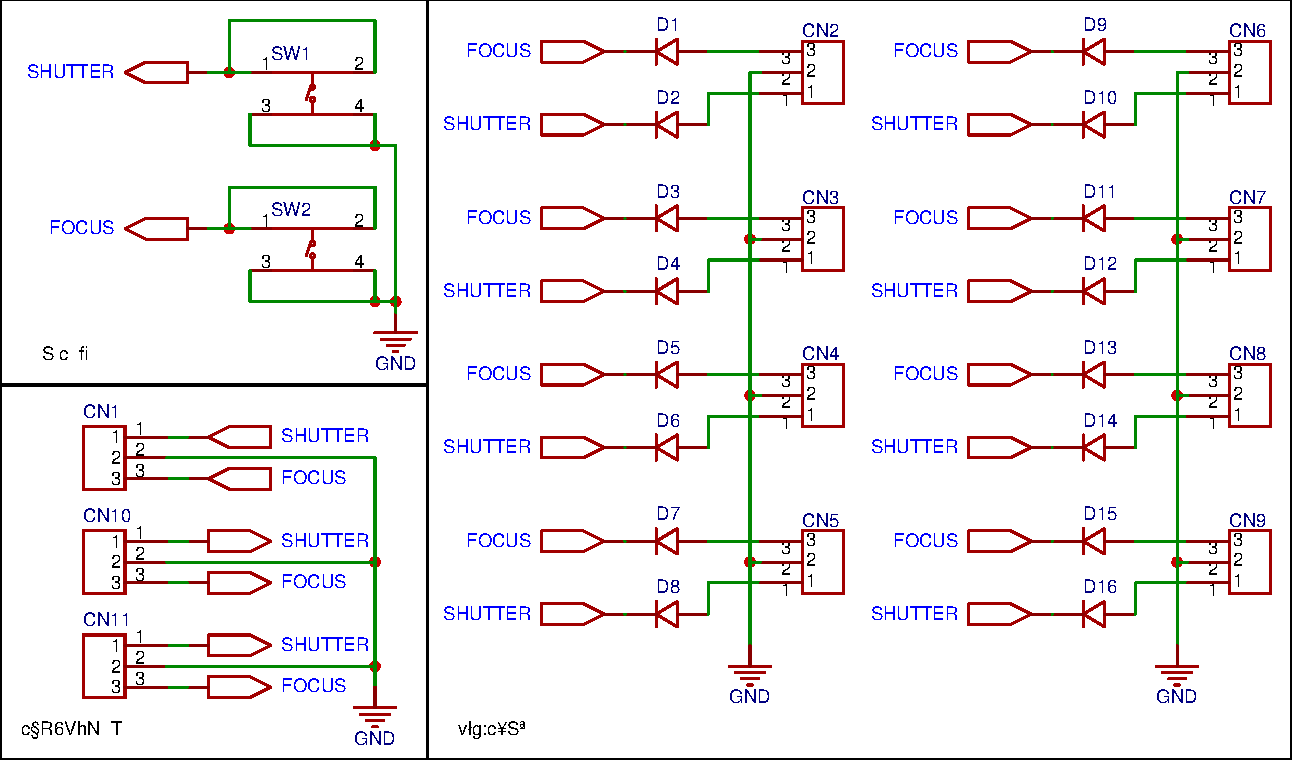
\includegraphics[width=\textwidth]{figures/passive_sync_schematic}
    \caption{被动控制器的电路原理图}
    \label{fig:passive_sync_schematic}
\end{figure}
\begin{figure}
    \centering
    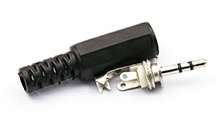
\includegraphics{figures/2.5mm}
    \caption{用于焊接的2.5mm插头}
\end{figure}
每个被动控制器的电路原理图如图\ref{fig:passive_sync_schematic}所示。

\chapter{主动同步控制器实现细节}

\paragraph{硬件}

\paragraph{软件}
在菜单的导航中,从左到右四个按钮的功能分别定义为:上一项,确认,下一项,返回;
在数值设置界面,这些按钮则分别为:减小,切换开启/关闭,增大,确认。

值得一提的是,在延迟设置的界面,用户可设置的最小分辨率为0.1毫秒,且最大范围为5秒,共50000个不同的设置值。
但本装置只有4个按钮,为了能快速设置到需要的值,本文设计了一种特殊的交互方式。
当用户按住增大按钮时,数值将不断增大,其增大的速度分为三个阶段:
在按钮按下时数值增大0.1毫秒,0.5秒内不再增大;
在0.5秒到2秒内,数值每0.1秒增大0.1毫秒;
在2秒后,数值与按住的时间呈二次函数关系:若当前按钮按住的时间为$2+t$秒,最大设定值为$m=5$秒,设定数值的增量在之前线性增加的基础上,再额外增加$m(t/10)^2$,
即在10秒内数值增量相当于整个设置范围。
如此即可兼顾定位的准确性和大范围移动的便利性。
在未来也可借助滚动编码器等额外硬件以提供更好的用户体验。
